\documentclass[jocse]{jocseart}

\usepackage{booktabs}
\usepackage[utf8]{inputenc}
\usepackage[english]{babel}

% Copyright
\setcopyright{jocsecopyright}
\jocseDOI{10.22369/issn.2153-4136/x/x/x }

\pagestyle{plain}
\pagenumbering{gobble}

\usepackage{cleveref}
\usepackage{todonotes}
\usepackage{graphicx}
\graphicspath{{./fig/}}
\DeclareGraphicsExtensions{.png,.pdf,.jpg,.jpeg}

\newcommand{\jk}[1]{\todo[inline]{TODO: #1}}
\newcommand{\ag}[1]{\todo[inline]{IDEA: #1}}
\newcommand{\kh}[1]{\todo[inline]{KH: #1}}

\begin{document}
\title{One Year HPC Certification Forum in Retrospective}

\author{Julian Kunkel}
\affiliation{%
  \institution{University of Reading}
  \streetaddress{}
  \city{Reading}
  \state{United Kingdom}
  \postcode{}
}
\email{j.m.kunkel@reading.ac.uk}


\author{Kai Himstedt}
\author{Nathanael Hübbe}
\affiliation{%
  \institution{Universität Hamburg}
  \streetaddress{}
  \city{Hamburg}
  \state{Germany}
  \postcode{}
}

\author{Weronika Filinger}
\affiliation{%
  \institution{EPCC, The University of Edinburgh}
  \streetaddress{}
  \city{Edinburgh}
  \state{United Kingdom}
  \postcode{}
}

\author{Jean-Thomas Acquaviva}
\affiliation{%
  \institution{DDN}
  \streetaddress{}
  \city{Paris}
  \state{France}
  \postcode{}
}


\author{Anja Gerbes}
\affiliation{%
  \institution{Goethe-Universität}
  \streetaddress{}
  \city{Frankfurt am Main}
  \state{Germany}
  \postcode{}
}

\author{Lev Lafayette}
\affiliation{%
  \institution{University of Melbourne}
  \streetaddress{}
  \city{Melburne}
  \state{Australia}
  \postcode{}
}

\renewcommand{\shortauthors}{J. Kunkel et al.}


\begin{abstract}

The ever-changing nature of HPC has always compelled the HPC community to focus a lot of effort into training of new and existing practitioners. Historically, these efforts were tailored
 around a typical group of users possessing, due to their background, a certain set of programming skills. However, as HPC has become more diverse in terms of hardware, software and 
 the user background, the traditional training approaches became insufficient in addressing training needs of our community. This increasingly complicated HPC landscape makes 
 developement and delivery of new training materials challenging. How should we develop training for users, often coming from non-traditionally HPC disciplines, and only interested in 
 learning a particular set of skills? How can we satisfy their training needs if we don't really understand what these are? It's clear that HPC centres struggle to identify and overcome the 
 gaps in users' knowledge, while users struggle to identify skills required to perform their tasks. 

With the HPC Certification Forum we aim to clearly categorise, define, and examine competencies expected from proficient HPC practitioners. 
In this article, we report the status and progress this independent body has made during the first year of its existence. The drafted processes and prototypes are expected to mature into a 
holistic ecosystem beneficial for all stakeholders in HPC education.
\end{abstract}

%
% The code below should be generated by the tool at
% http://dl.acm.org/ccs.cfm
% Please copy and paste the code instead of the example below.
%
\begin{CCSXML}
\end{CCSXML}



\keywords{}

\maketitle

\section{Introduction}

There is a generally accepted set of skills and competencies necessary to efficiently use HPC resources. 
This skill set depends on the role and domain of the practitioner but also on the available infrastructure of the center providing the computing resources.
For example, a scientist needing to run an application on a specific machine may need basic skills in Linux, MPI, environment modules, and knowledge about the batch scheduler, e.g., Slurm.
Now rather than providing that scientists with a list of instructions to be followed in a copy and paste fashion or a never-ending list of things they should know, we want them to understand each of the required steps without having to learner everything about it, but at the same time understand how it fits into the bigger picture of using an HPC system. 
For instance, understanding Slurm is a good example of a very fine-grained skill that fits under a more generic skill defined as "resource management", illustrating concepts across the rich variety of available resource managers.

Most institutions operating HPC systems offer regular training events focusing on general aspects of their supercomputer's hardware architecture, software stack, application development environment  and various tuning and debugging tools.   
It is understandable why the materials they are geared towards the special demands of the institutions they support and its specific HPC environment. 
The problem is that teaching content typically covers only a small part of basic HPC skills necessary to use other HPC systems. 
This approach of teaching only specific implementations, tools or workflows, instead of concepts behind them makes a move to a different system or tool unnecessary complicated. 
Narrowing the scope of training events make sense from the HPC provider perspective, but is not very conducive to development of more comprehensive learning environment that provides assessment and certifies the newly acquired skills. So although, certificates are used widely in IT industry to verify certain knowledge, until now there was no similar approach for HPC training. 
It is, however, clear that a certification scheme could address some of the challenges stemming from the constantly growing training needs of our community,  

This article describes the current status of the certification program initiated by the HPC Certification Forum.
Our previous work provided a brief overview of the evolution from the project that sparked the HPC Certification Forum \cite{TAHCPKHHSS19} while this article provides details on adopted mechanisms and design decisions.

The article is structured as follows:
First, in \Cref{sec:forum} we introduce the HPC Certification Forum and the certification program. 
Then, an overview of the status is given in \Cref{sec:status}, followed by the organisation of competencies discussed in \Cref{sec:skills}.
This leads to the proposal for the certification process in \Cref{sec:certification}.
In \Cref{sec:ecosystem} the whole learning ecosystem is described.
Related work is presented in \Cref{sec:related}.
Finally, the article is concluded in \Cref{sec:conclusion}.

\section{The HPC Certification Forum}
\label{sec:forum}

The HPC Certification Forum (HPCCF) has the role of a (virtual) central authority to curate and maintain a certification program.
The program consists of the definition of competencies, the creation of certificates, and the examination of practitioners to attest that they possess certain competencies.
Moreover, the forum supports tools and an ecosystem around the competencies.

The HPCCF aims to support existing activities and complements them by providing a unified and clear way of mapping out the relevant HPC competencies for practitioners.
Thus, the HPCCF does not regulate the content of training material; we purposely separate the definition of skills and certificates with their examinations from content delivery.
Similarly, the program does not prescribe a curriculum or any fixed order by which skills need to be obtained.

The forum is organized using a Webpage\footnote{http://hpc-certification.org} and utilizes Slack\kh{Vorschlag: kurzen Hinweis zu Slack ergänzen "...  cloud-based set of proprietary team collaboration tools ..." bzw. Link auf die Website} for communication and monthly meetings.
Members are organized in different roles:
Anyone can become an associate member in the HPCCF free of charge -- e.g., observing the status, being listed on the webpage.
Full members must actively contribute to the program to some extent and have voting rights for the roles of the steering board.
The steering board directs the overall activities and is organized in different responsibilities, i.e., into topic-specific chairs.


\section{Overview of the Activities}
\label{sec:status}

During the first year of the existence of the HPCCF, the discussion within the forum and with partners has lead to the establishment of various processes and prototypes for technical tools that are described in the following briefly.
Further details of the overview are provided in subsequent sections.

\paragraph{Management}
At ISC-HPC 2018, the first steering board had been elected.
We established communication channels via webpage, email and Slack for regular discussion.
Slack is also used to conduct our monthly open meetings between members and the steering board.
At beginning we used video conferencing tools, but found that the chat provides a more inclusive discussion and the asynchronous nature is more productive.
We also established relations with various stackholders involved in HPC education growing the participation in the forum.
Meeting notes with action items are extracted from Slack and documented using Google Doc\kh{Vorschlag: kurze Info zum Tool bzw. Link (wie bei Slack) ergänzen}.

Note that until now contributions of members are voluntarily and follow the schedule as agreed between the contributor and the HPCCF board.
We manage the prospect contributions in a Trello board\kh{Vorschlag: kurze Info zum Tool bzw. Link (wie bei Slack und Google Doc) ergänzen (Trello kennt ja nicht unbedingt jeder Leser); der Begriff "collaborative" sollte irgendwo untergebracht werden}; each member can manage its own card.

\paragraph{Technical}\kh{"Management" (oberhalb) finde ich auf der Ebene alleinstehend gut, "Technical" etwas zu kurz, Vorschlag: "Technical Tasks" (o.ä.)}
According to our goals, we address 1) the definition of competencies; 2) the creation of certificates; 3) the examination of practitioners; and 4) an ecosystem of tools supporting them.

For all these sub-goals we made substantial progress.
While the definition and organization of competencies was the main focus, we prototyped various tools and processes that embed the competencies into the wider education ecosystem.

Firstly, we finalized the templates for the description of a competence considering pedagogic literature from higher education.
We are still working on mapping out all relevant competencies, but included also new topics that will be covered in the first version of the certification program.

The definition of the competencies covered by the program is version controlled with Git.
The competencies are available in XML and Markdown format.
A Wiki allows to edit the competencies and simplifies access for non-technical users.
A navigable JavaScript representation of the skill tree is available that can be customized for the HPCCF but also for end-users.

Prototypical processes and tools have been developed and deployed for curation of the examination questions and for conducting an online multiple-choice examination.

\section{Skills}
\label{sec:skills}

A skill is defined as a set of competencies (learning outcomes) and some metadata.
This model can be compared to the classification of school knowledge, for example, the skill with the short name “addition” could describe the math skill of being able to add numbers successfully.\kh{ich halte ein prägnantes und gutes Beispiel hier für wichtig. Ohne den Übergang zum Expert Level gefällt mir die "Addition" auch gut, aber der Übergang zu "Expert" mit dem Addieren mehrerer Zahlen ist zwar auf abstrakter Ebene ok, aber doch etwas weit entfernt von der Praxis; so spontan fällt mir als analoges alternatives Beispiel aus dem Bereich der Geometrie das Zeichnen einer Geraden mit dem Lineal ("Basic Level") oder die Konstruktion eines Sechsecks mit Zirkel und Lineal ("Expert Level") ein}.
Within a single skill, there can also be multiple levels (basic, intermediate, expert level) building upon each other that distinguish the expertise further.
We expect that practitioners acquire the lower levels before progressing to more complex levels.
In our addition example, \textit{basic level}, for example, may mean to be able to add two positive numbers while the \textit{expert level} of that skill could indicate to be able to add multiple numbers.

The basic level should cover the most relevant aspect of the skill, i.e., needed by anyone that uses the skill, the intermediate level (used for common exceptional cases) and expert levels (used in special circumstances)  are needed only for a subset of users.
Typically, an institution has only few experts (if one at all).

The skills are organized in a tree that serves the purpose to organize and structure the skills from a coarse-grained to a fine-grained representation allowing users to browse the skill based on the semantics.
The root level of our current skill tree is shown in \Cref{fig:skill-tree}; we aim to finalize the tree this year.
The basic idea is that the skills from the root level enable navigation by providing an indication about their scope, e.g., are they core knowledge, dealing with the usage of HPC environments, or about programming.
This should allow the user to rapidly drill into the skill representation.
The closer a skill is to the root, the more abstract it is defined, while leaf nodes cover the knowledge for the specific skill.


As the tree serves the purpose to organize the skills, there can also be references from one branch to a skill in another.
This import allows to reuse the definitions of the skills while still allowing users to navigate the tree according to the semantics.

\begin{figure*}[tb!]
	\centering
	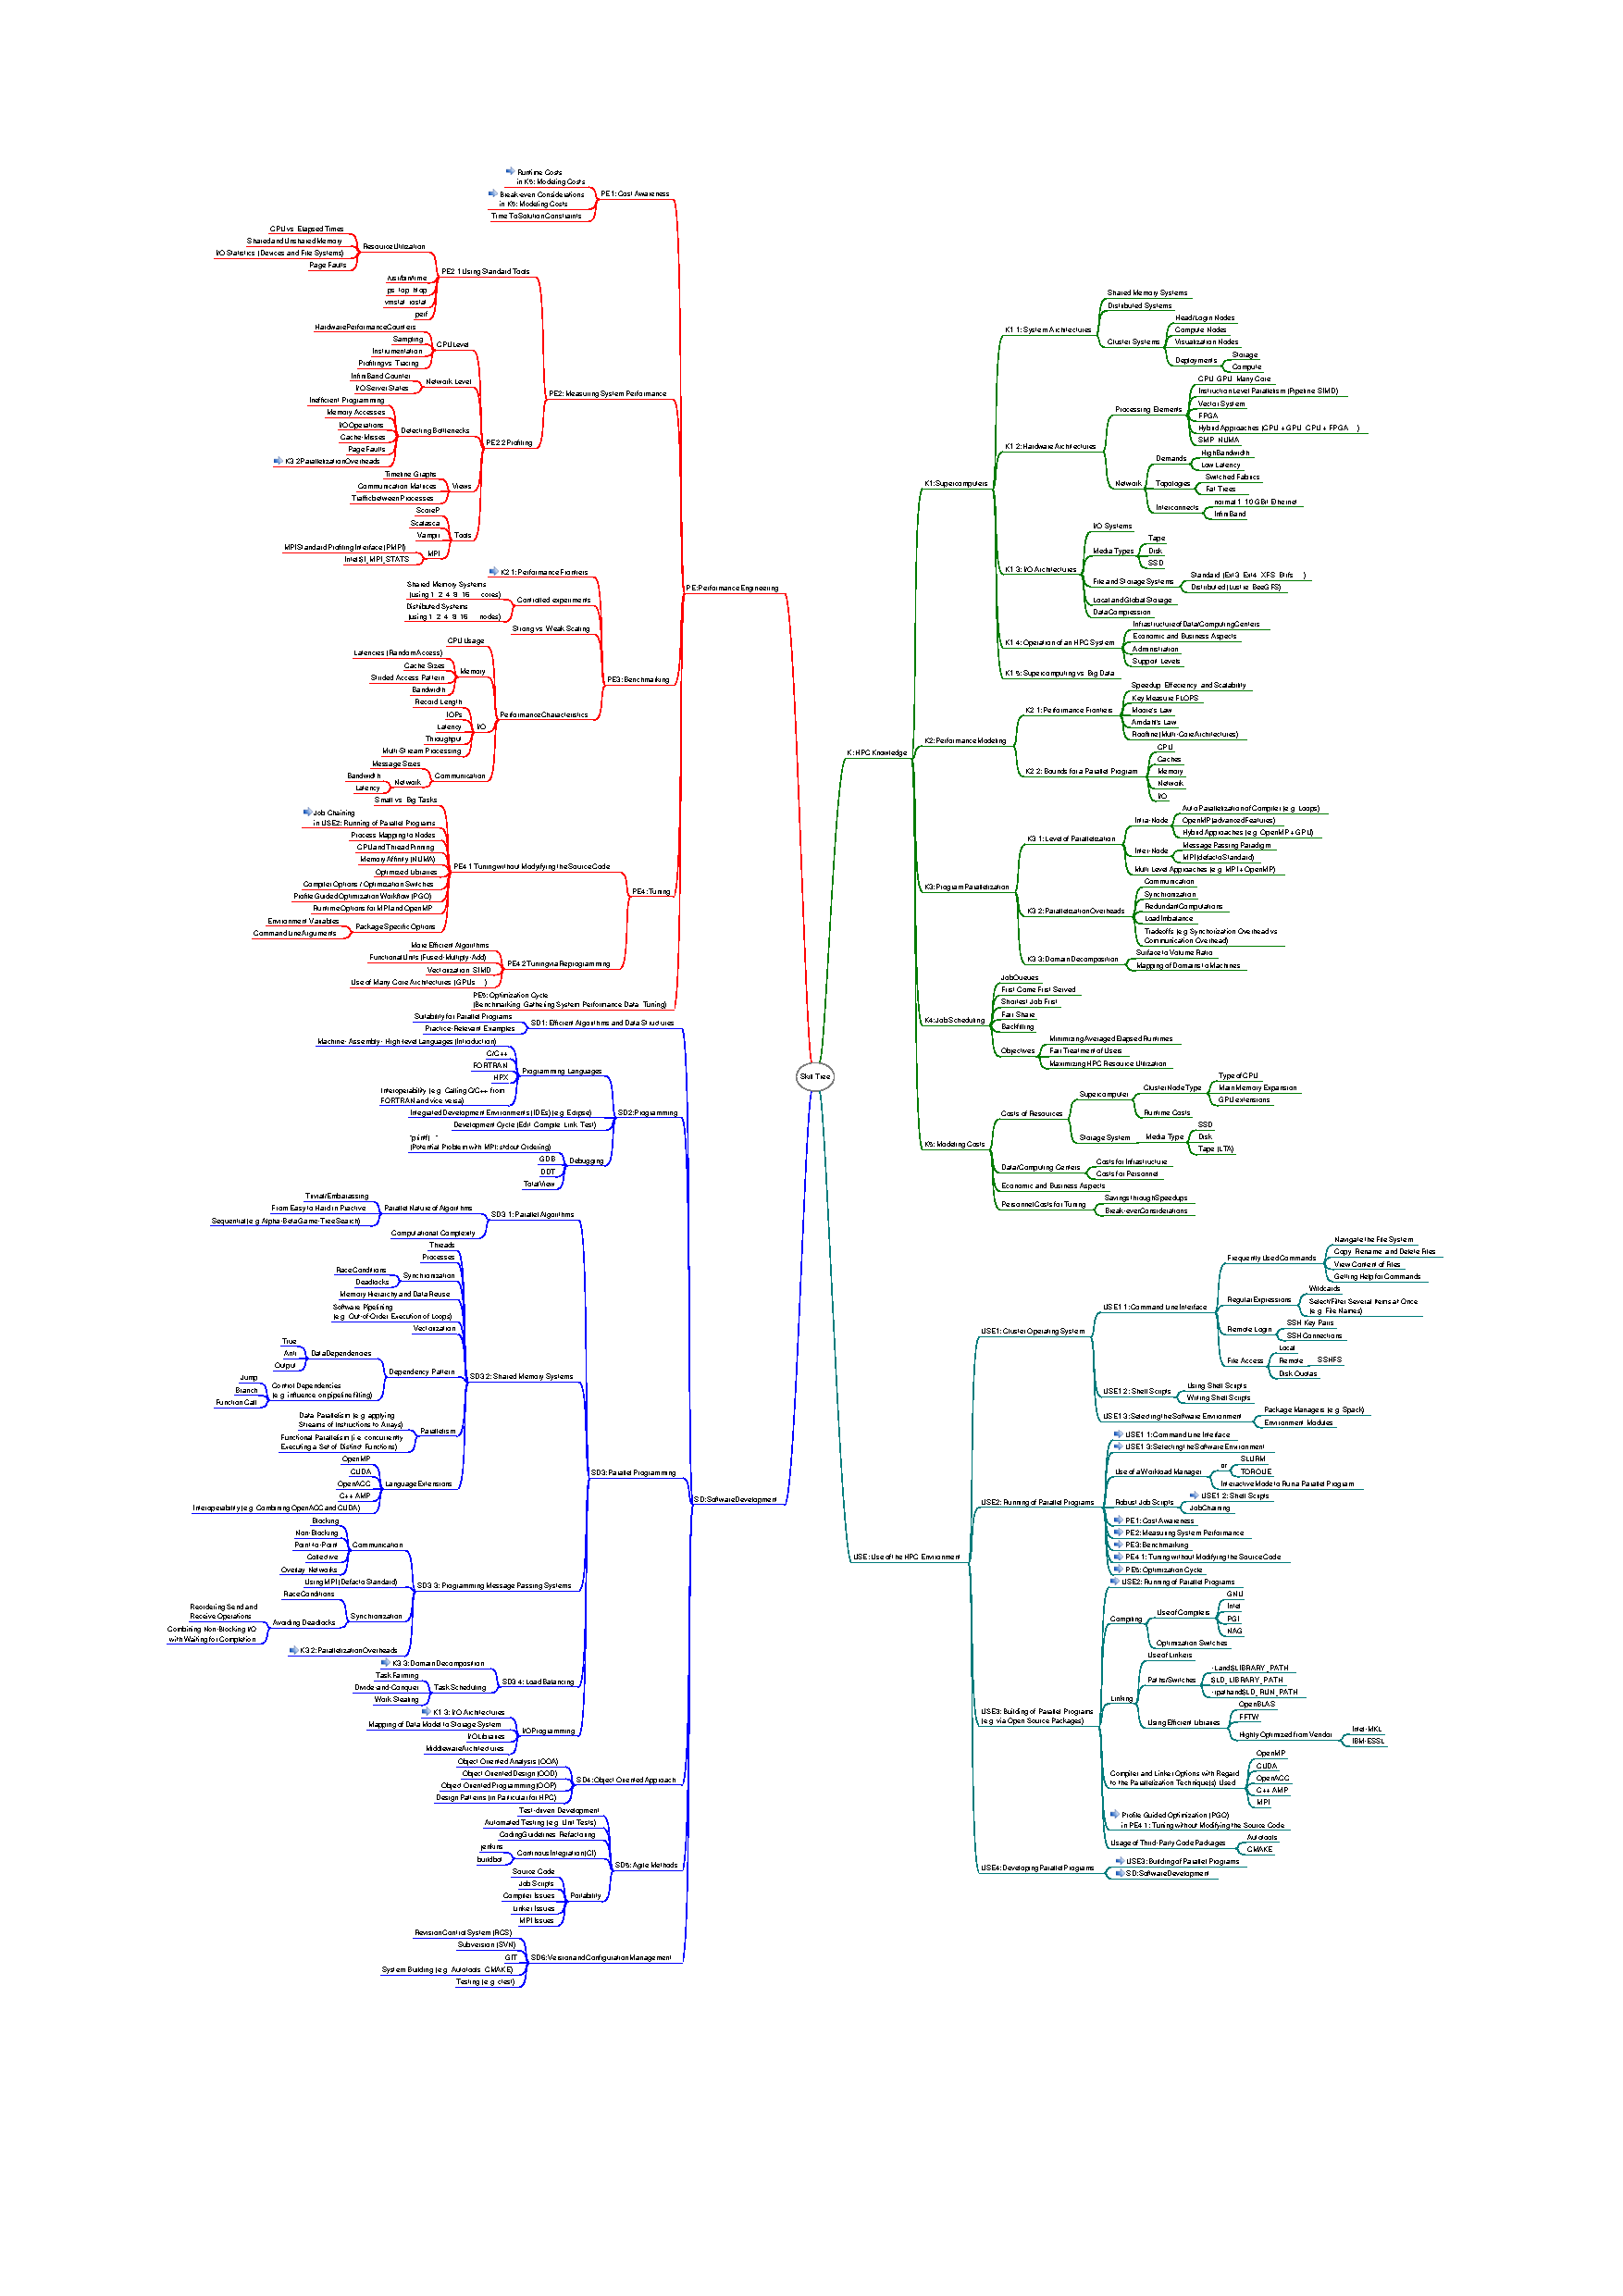
\includegraphics[width=15.0cm]{skill-tree}
	\caption{Skill tree top level competencies with an expansion of PE4}
	\label{fig:skill-tree}
\end{figure*}

\subsection{Description of a skill}

Each skill on the tree and even the inner nodes are described in more detail as follows:

\begin{itemize}
  \item \textbf{ID}: ID according the organization in the skill tree. The last character indicates the level of the skill (Basic, Intermediate, or Advanced).
  \item \textbf{Name}: A speaking name for the skill.
  \item \textbf{Background}: Provides brief information motivating the need for the skill and how this skill fits into the skill tree; what is the bigger picture.
  \item \textbf{Aims}\footnote{The definition of aims and outcomes follows literature for higher education \cite{williamson2011good} and \url{https://www.heacademy.ac.uk/system/files/assessment-learning-outcomes.pdf}.}: They serve as broad purposes and are generally a statement of the intentions of the skill.
  They are not the statements of what a practitioner will learn or do.
  At a basic level, aims are trying to answer two questions: What is the purpose of this skill?
  What is the skill trying to achieve?
  \item \textbf{Learning outcomes (LOs)}: Defines briefly what practitioners will know and learn.
  The objected are statements what prospect learners are able to do, they should
  describe or define an action be clearly stated be measurable/quantifiable to some extent by using action words.
\end{itemize}

On the leaf level, a skill is fine-grained and orthogonal to other skills -- we scope the level of detail here to be able to be taught in a 1.5 hour lecture up to a 4 hour workshop.
We believe this is a good granularity as it allows practitioners to cherry-pick the relevant skills and lecturers and examiners to prepare small lectures with well-defined content.
\ag{change sentence because provided that provide - \\
Instead: For technology-dependent skills on leaf level (e.g., a specific file system or workload manager), often introductory skills are provided that provide the foundation to many specialized skills each representing a specific hardware or software technology.\\
write it this way: For technology-dependent skills on leaf level (e.g., a specific file system or workload manager), often introductory skills are provided that contribute to the foundation of many specialized skills each representing a specific hardware or software technology.
}
The aggregation within the tree is similar to the aggregation found in education as part of “individual teaching events”, “those specified for modules or short courses”, and “those specified for whole degree programmes” \cite{hussey2008learning}.
While that Hussey et al. conclude that LOs on the coarse grained level are not useful for high-level education, we use a similar concept, but relax the granularity/abstraction level of the learning outcome.\kh{den Satz habe ich nicht genau verstanden; als Leser würde ich mir die Kurzbegründung wünschen, die Hussey et al. für ihre Feststellung anführen}

\subsection{Skill Examples}

Next, we present a generic skill that describes an inner-node in more details.
\ag{change sentence because delivery and deliver in one sentence - 
There is no actual delivery as a module or teaching event to deliver the content, it serves the purpose to inform the practitioner about the importance of the skill.
}
\begin{itemize}
  \item \textbf{ID}: USE4.2-B
  \item \textbf{Name}: Executing parallel applications
  \item \textbf{Background}:
  Parallel computers are operated differently than a normal PC, all users must share the system. Therefore, various operative procedures are in place. Users must understand these concepts and procedures to be able to use the available resources of a system to run a parallel application. Moreover, individual solutions can often be found in a specific system.
  \item \textbf{Aim}: To enable practitioners to comprehend the concepts and procedures for running parallel applications in HPC environments.
  To use the system to run and monitor the execution of parallel applications on the HPC system.

  \item \textbf{Learning outcomes}:
    \begin{itemize}
    \item explain the concepts and procedures for resource allocation and job execution in an HPC environment
    \item run interactive jobs and batch jobs
    \item comprehend and describe the expected behavior of job scripts
    \item change provided job scripts and embed them into shell scripts to run a variety of parallel applications
    \item analyze the output generated from a job scheduler and describe the cause of typically generated errors
    \end{itemize}
\end{itemize}

\ag{When I was reading the "learning outcome" of USE4.2B, another category came to mind: 
How to write job scripts? How to batch use?
So why not create a case where the learning outcomes overlap?
Since you did the skill examples with USE4.2 in 4.2, I would not do "Figure 1" with extension of PE4 but USE4.
Then you can always look there.
}

The next leaf-level skill describes how workload management works in general in HPC regardless of the specific software that implements such concepts.
It is intended that the aim and outcomes from the parent skill above are covered to some extend and refined into specifics.


\begin{itemize}
  \item \textbf{ID}: USE4.2.1-B
  \item \textbf{Name}: Workload manager introduction
  \item \textbf{Background}: There is a wide range of different workload managers in use. This skill covers generic and widely used concepts.
  \item \textbf{Aim}: To enable practitioners to comprehend and describe the basic architecture and concepts of resource allocation for an HPC system.
  \item \textbf{Learning outcomes}:

  \begin{itemize}
  \item comprehend the exclusive and shared usage model in HPC
  \item differentiate batch and interactive job submission
  \item comprehend the generic concepts and architecture of resource manager, scheduler, job and job script
  \item explain the role of environment variables as a means to communicate
  \item comprehend accounting principles
  \item explain the generic steps to run and monitor a single job
  \end{itemize}
\end{itemize}


The following skill describes a leaf-level skill for the usage of Slurm in\kh{at} the basic level.
While there is no formal dependency to the introduction (skill USE4.2.2-B), it is expected that practitioners have obtained the other skill before learning this one.

\begin{itemize}
  \item \textbf{ID}: USE4.2.2-B
  \item \textbf{Name}: Slurm Workload manager
  \item \textbf{Background}: Slurm is a widely used open-source workload manager providing various advanced features\kh{Vorschlag: einige der Highlights anführen: "... , like ..."}.
  \item \textbf{Aims}:
  \begin{itemize}
    \item To enable practitioners to use relevant tools to run and monitor parallel applications using Slurm.
    \item To enable practitioners to comprehend and describe the basic architecture of Slurm and the suite of tools.
  \end{itemize}
  \item \textbf{Learning outcomes}:
  \begin{itemize}
  \item run interactive jobs with salloc, a batch job with sbatch
  \item explain the architecture of Slurm, i.e., the role of Slurmd\kh{Slurmd haben wir beim "Basic Level" bisher nicht vorgesehen}, srun and the injection of environment variables
  \item explain the function of the tools: sacct, sbatch, salloc, srun, scancel, squeue, sinfo
  \item explain time limits and the benefit of a backfill scheduler
  \item comprehend that environment variables are set when running a job
  \item comprehend and describe the expected behavior of a simple job scripts\kh{typo?}
  \item comprehend how variables are prioritized when using command line and a script
  \item change a provided job template and embed them into shell scripts to run a variety of parallel applications
  \item analyze the output generated from submitting to the job scheduler and typically generated errors
  \end{itemize}
\end{itemize}

\ag{I could put my slide set online and show the skill tree for the slide set. An example could be shown, there the content described in a skill tree are also explained in slide sets.
Everything under USE 4.2.2 B, I have explained it in my slide set under "Slurm Usage on Goethe HLR cluster".
\\
What I have found and would like to try it out:  http://xlong88.github.io/draw-binary-tree-latex/
Create recursive and automatically a Binary Tree with Tikz and Tikz-qtree.
If we can do it generically then I will be one step ahead with my skill tree for the slide set.
}

As you can see from the definition of the skill, these learning outcomes are focusing on the core needs to actually use Slurm effectively.
An intermediate skill could, e.g., add reservations.

%\begin{itemize}
%  \item \textbf{ID}:
%  \item \textbf{Name}:
%  \item \textbf{Background}:
%  \item \textbf{Aim}:
%  \item \textbf{Learning outcomes}:
%\end{itemize}


\section{Certification}
\label{sec:certification}

A certificate shall attest a user the expertise in the covered skills.
Ensuring the integrity of a certificate is an important aspect, i.e., we must check that the learning outcomes of the covered skills are achieved and prevent self-cheating or dishonesty.

Students can always cheat an examination -- the risk depends on the type of exam and methods used for the assessment.
As we want to enable a cost-effective assessment (free for the practitioner), we chose an online examination.
This increases the opportunity for cheating \cite{rowe2004cheating} but we deploy several  strategies that aim to minimize the risk of self-cheating as raising awareness, a question pool, and delay.
Since knowledge can age, the month and year an examination took place is also indicated.
As certificates bundle multiple skills together as examination of a single fine-grained leaf-level skill would be too easy for short-term memorization and prone to self-cheating.
We believe the incentive to deliberately fake the assessment, e.g., by having the exam filled by someone else, and thus, being awarded a certificate is low.
Therefore, we address this only in a lightweight fashion.

A process has also been created for prospect contributors of examination questions.
The questions are the only proprietary component for the HPCCF using restrictive license terms for authors while we give credit to them.
We considered this necessary to minimize the establishment of solution databases; we omit further details here.

We discuss the prototypical process that we implemented for conducting examination in the following.

\subsection{Examination Process}

The examination can be started by users any time but upon submission a delay is employed.
Firstly, a user has to register for the examination using name and email address and optional affiliation.
On the webpage, the process is explained, together with privacy policies.
Further, a paragraph provides the integrity policy defining cheating and encouraging honesty.
Practitioners are asked to opt-in the policy statement.
With the registration, we generate an encrypted token on the server that is returned to the user by email.
At this stage, we do not store any information about the user on the server.

The email contains a link that will start the examination.
The user chooses to start the examination by clicking on the link; then the information about the user and the time of starting the examination is stored in a temporary database.

The summative assessment itself is conducted using multiple choice questions.
Therefore, for each skill, we will be developing a pool of questions but also allow contribution of questions.
A question has more possible answers (e.g., 10) -- the practitioner has to select if each  statement is true or false.
An examination consists of randomly selected questions and five answers per question are selected.

Once the user submits the exam results, all selected answers are stored on the server for validation -- which is done manually at the moment.
If the user meets the criteria to pass (typically 70\% correct selection), a certificate is issued and send to the user by email.
We then delete all personal information about the user from the server but preserve the affiliation and the raw responses.
The affiliation is used for promotion purposes while the raw responses will be analyzed to optimize the questions.
For example, when we identify that most users make a particular mistake, this may be an indication that the question or answer is ambivalent and needs to be improved.

If the user didn't meet the criteria to pass, we will inform him about the rough score obtained.
The user can retry to obtain the certificate after a cooldown period (typically one week) but not immediately to prevent success via brute force methods.
To enforce this, we keep the information about the date the exam was conducted linked to his name and email.

As the sole purpose of the multiple choice questions is the examination, we will not reveal which questions are answered correctly.
We assume that high quality training material for individual skills will offer multiple choice questions that serve the purpose of feedback which promotes learning  \cite{epstein2002immediate}.

\subsection{Certificates}

Upon successful assessment, a certificate is awarded, it consists of two parts:
A PDF with the key information needed for a meaningful certificate (for a draft, see \Cref{fig:awardedCertificate}).
The name and identifier for the certificate is found in the center and below (here 4711 and “the basic certificate”).

Secondly, a text file is given to the user that provides the same information.
It is PGP signed using the private key of the HPC Certification Forum to allow verification with the published\kh{"published" wäre redundant} public key.
It also contains a verification URL that can be given to a third-party allowing verification of the information.

The file looks as follows:
\begin{verbatim}
-----BEGIN PGP SIGNED MESSAGE-----
Hash: SHA512
HPC Certification Forum Certificate
This text confirms that "Julian M. Kunkel" has
successfully obtained the certificate
"The basic certificate" (id: 4711) at 02/2019.
Verification URL: https://hpc-certification.org/[...]
-----BEGIN PGP SIGNATURE-----
[...]
-----END PGP SIGNATURE-----
\end{verbatim}

\begin{figure}
  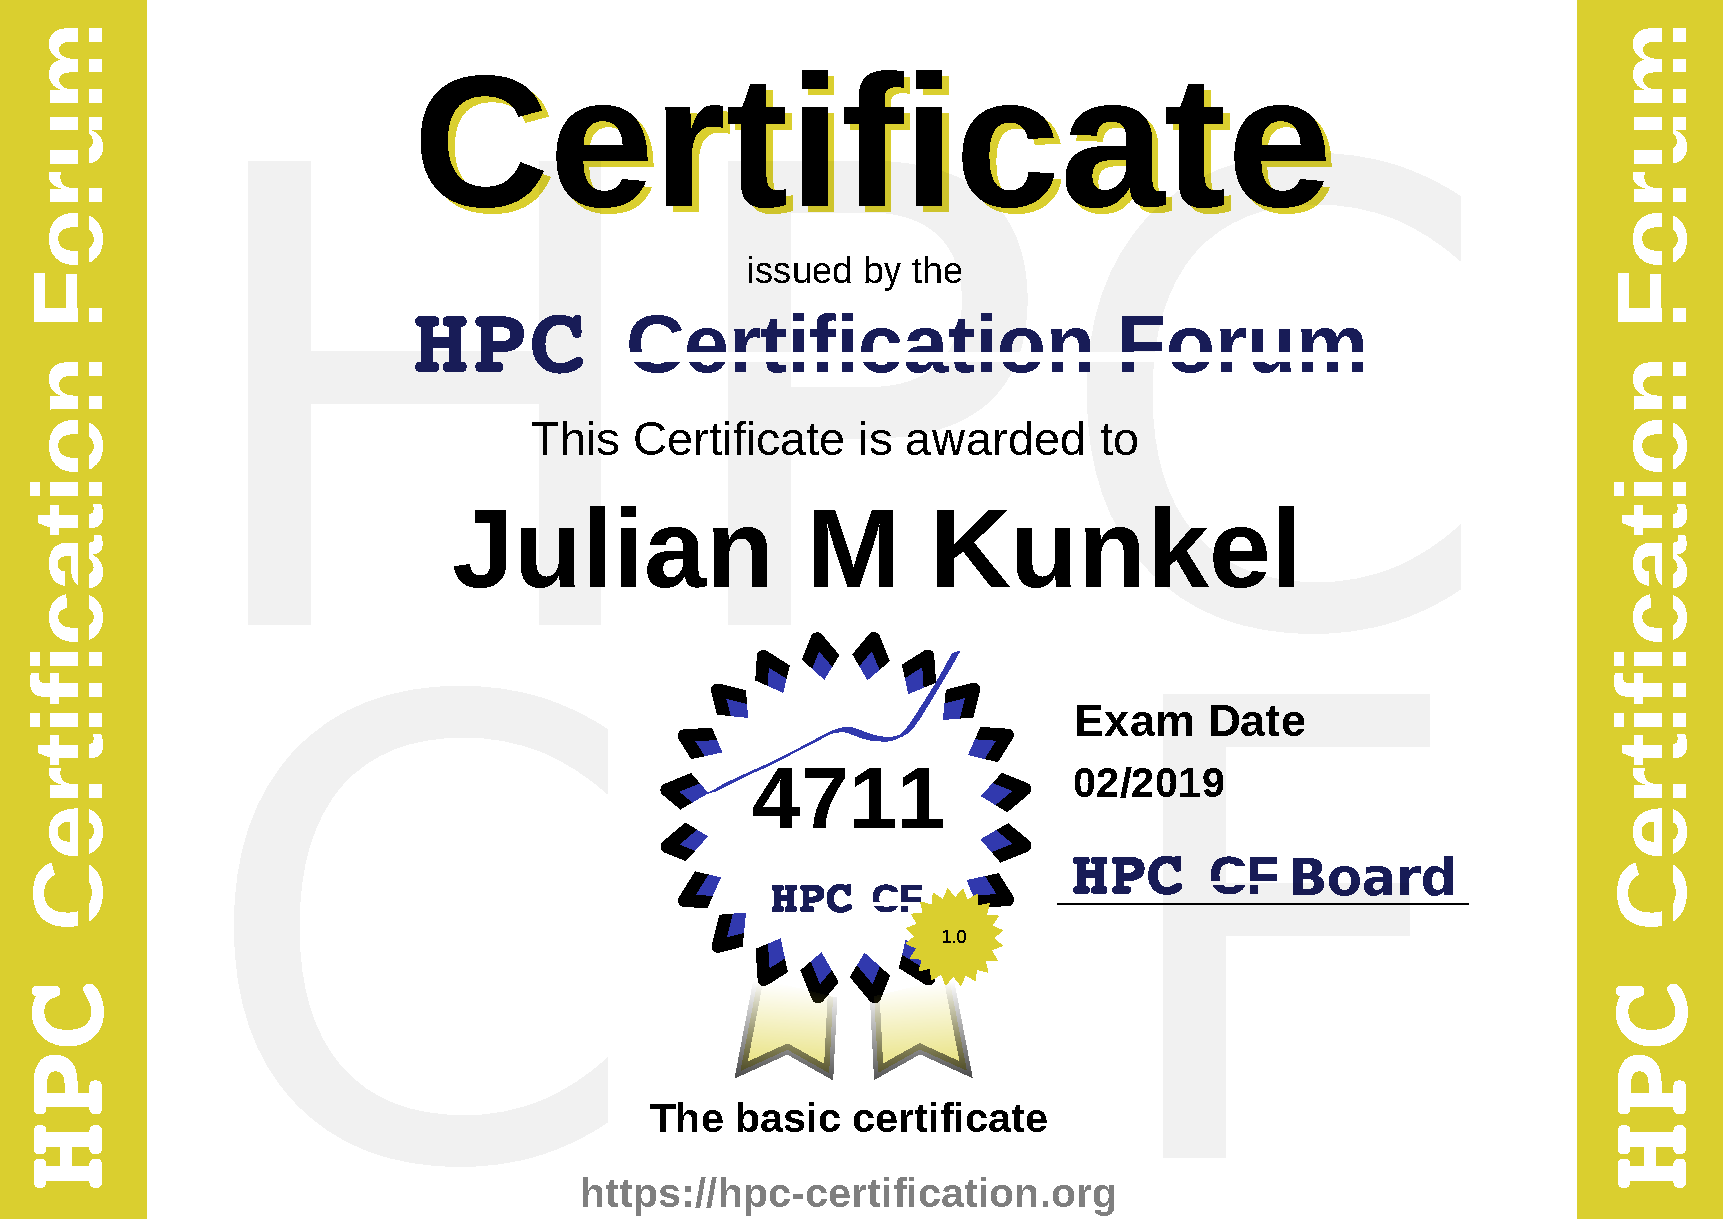
\includegraphics[width=0.48\textwidth]{JulianMKunkel}
  \caption{Draft for an awarded certificate}
  \label{fig:awardedCertificate}
\end{figure}
\kh{Vorschlag: "The basic certificate" ist ja sehr generisch und verlangt vom Leser (vermeidbares) Abstraktionsvermögen; ein prägnantes und praxsinahes Beispiel erscheint mir hier geeigneter}

\section{Ecosystem}
\label{sec:ecosystem}

We encourage the development of an ecosystem around the HPC classification, we are supporting training and tool development.

\subsection{Training Delivery}

The HPC Certification Forum is not developing training material directly or competing with providers of training material.
However, we support individuals and institutions by endorsing and promoting their training materials and courses in two ways.

Firstly, an author of training material is allowed to indicate on the training material itself or on promotional material the fact
which skills are covered by the material completely or partially.
We provide a seal that can be used for that purpose (see \Cref{fig:seal-teaching}).
The reference to the HPCCF and the seal can be used free of charge under the condition that the developer of the training material
registers a link to the material or course and their\kh{Plural hier beabsichtigt (Bezug?)} email address on our webpage using an online form.
That way, the HPCCF is informed about the usage of the seal.

Secondly, we will link on our webpage the endorsed training material for the individual skills and certificates.
By using JavaScript and dynamic webpage we will provide various views on the skills with and without links to suitable training materials.

Note that we are not intending to verify the correct usage of the skill explicitly.
However, in case the training material or course doesn't deliver the expected material practitioners may complain and we will remove the training material from our webpage.

We expect that this strategy will lead to the availability of good free training material for most skills while companies and individuals can still charge for effective training courses.
Ultimately, the resulting training material will complement each other leading to a rich variety of content suitable for each individual practitioner, e.g., addressing different learning styles and languages.

\begin{figure}
  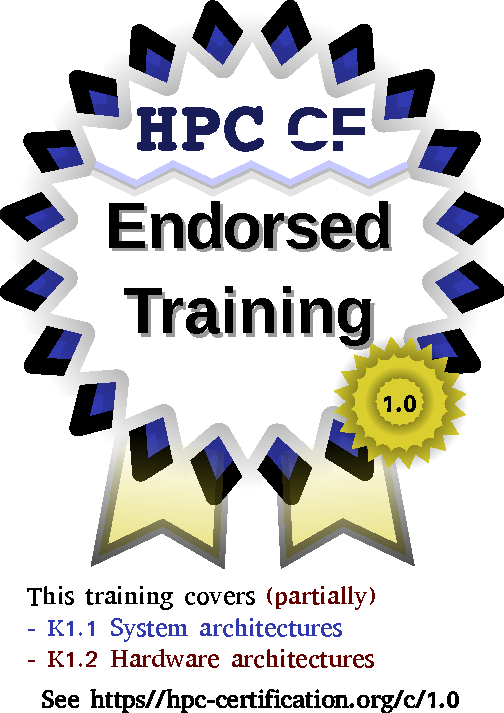
\includegraphics[width=0.3\textwidth]{certified}
  \caption{Draft for the seal for teaching material}
  \label{fig:seal-teaching}
\end{figure}


\subsection{Navigation}\kh{Vorschlag Unterkapitel in "Results" umbenennen oder an anderer Stelle aus "Erwartungsgründen" ein "Results"-Kapitel ergänzen (am besten natürlich auf der Hauptgliederungsebene, aber das wird vermutlich schwierig werden)}
%\paragraph{Navigation}
Thanks to the contributions of the PeCoH project, a JavaScript prototype enables the embedding of a navigable skill tree into a webpage.
The script can be used by different stackholders to present their own view on the skill-tree.
By view we mean the selection and organization of the skills, and the additional information provided when navigating the tree.
For instance, you could have a tree for a specific scientific domain, for a specific data center, or even for the role of the tester of a specific application; it could indicate which skills are mandatory or beneficial for these use cases, providing links to training material or adding further supplementary information.


\section{Related Work}

\label{sec:related}

\jk{Please everyone!}

Relevant work can be classified into approaches to establish a curriculum or the creation of teaching material.
In academia, individual universities offer their own curriculum around scientific computing and HPC, covering theoretical aspects like the software development of numerical applications.
They are not tailored to the needs of a practitioner to actually use HPC systems effectively.
Data centers offer their own material and courses to support their own users.
Several projects address the generation and sharing of teaching material for HPC.
The EuroLab-4-HPC project establishes training in form of (online) courses\footnote{\url{https://www.eurolab4hpc.eu/}}.
The Barcelona Supercomputing Centre (BSC) aims to develop a professional training curriculum \cite{sancho2016bsc}.
The virtual organization XSEDE\footnote{\url{https://portal.xsede.org/web/xup/training/overview}} provides an online system to train the usage of an HPC system, structuring the corresponding information on their website into major topics like “Getting Started”.
The user can navigate the topics and receive further information.

\section{Conclusion}
\label{sec:conclusion}


This allows the re-use of existing content but also allows to create a new ecosystem in which HPC centers or commercial companies could offer the best teaching material.
Teaching material should be marked to indicated which skills it covers.
In the future, the program may provide means to register and reference existing content of third-parties allowing users to browse the skills and navigate to teaching material.


\subsection{Benefits}

HPC practitioners
Increase motivation to participate
(Certificates are recognized in CV)
Validate knowledge via tests
Browse of relevant competencies
Identify recommended and required skills
Compare teaching offers across sites
Data centers

Increase sharing of teaching materials
Documentation of taught skills simplified
Identify missing teaching activities
Tailor skill-tree specifically to users
Correlate lack of skills with efficient us\kh{diese Subsection ist vermutlich noch in Arbeit; Groß-/ Kleinschreibung?}

Making clear what skills are required of or recommended for a competent HPC user would benefit both the HPC service providers and practitioners.
Moreover, it would allow centres to bundle together skills that are most beneficial for specific user roles and scientific domains.
From the perspective of content providers, existing training material can be mapped to competencies allowing users to quickly identify and learn the skills they require.
Finally, the certificates recognized by the whole HPC community simplify inter-comparison of independently offered courses and provide additional incentive for participation.





\appendix

\begin{acks}
\small
We are thankful for the contributions and discussions with the members of the HPCCF and for the contributions made by the PeCoH project.
\jk{TODO}
PeCoH was supported by the German Research Foundation (DFG) under grants LU 1353/12-1, OL 241/2-1, and RI 1068/7-1.
\end{acks}

\bibliographystyle{ACM-Reference-Format}
\bibliography{bibliography}

\end{document}
